 % 五号字体,开明式标点处理,不设置默认字体
\documentclass[UTF8, 12pt, punct=kaiming, fontset=none]{article}
\usepackage[UTF8]{ctex}
\usepackage{fontspec}
\usepackage{float}
\usepackage{graphicx}
\usepackage{subcaption}
\usepackage{pgf-umlsd}
% 品红色链接和注释
% \usepackage[colorlinks=true, linkcolor=magenta, citecolor=magenta, urlcolor=magenta]{hyperref}
% 黑色链接和注释
\usepackage[colorlinks=true, linkcolor=black, citecolor=black, urlcolor=black]{hyperref}
\usepackage{geometry}
\usepackage{fancyhdr}
\usepackage{caption}
\usepackage{framed}
\usepackage{titlesec}
\usepackage{ragged2e}

\graphicspath{{figures/}}

% 字体
\IfFontExistsTF{Source Han Serif SC}
{
    \setCJKmainfont{Source Han Serif SC}
}
{
    % GitHub Actions
    \setCJKmainfont[
        Path=. ./fonts/ ,    
        Extension = . otf ,
        UprightFont = *-Regular ,
        BoldFont = *-Bold
    ]{SourceHanSerifSC}
}
\IfFontExistsTF{Source Han Sans SC}
{
    \setCJKsansfont{Source Han Sans SC}
}
{
    % GitHub Actions
    \setCJKsansfont[
        Path=. ./fonts/ ,    
        Extension = . otf ,
        UprightFont = *-Regular ,
        BoldFont = *-Bold
    ]{SourceHanSerifSC}
}
\IfFontExistsTF{DejaVu Sans}
{
    \newfontfamily\ds{DejaVu Sans}
}
{
    % GitHub Actions
    \newfontfamily\ds[
        Path=. ./fonts/ ,    
        Extension = . ttf ,
        BoldFont = *-Bold ,
        ItalicFont = *-Oblique ,
        BoldItalicFont = *-BoldOblique
    ]{DejaVuSans}
}
%\newfontfamily\cm{CMU}

% 图表标题字体
\DeclareCaptionFont{captionfont}{\ds}
\captionsetup[table]{font=captionfont}
\captionsetup[figure]{font=captionfont}


% 布局
\geometry{a4paper, left=2cm, right=2cm, top=2.5cm, bottom=2.5cm}
\setlength{\headheight}{25pt}

% 页眉页脚
\pagenumbering{arabic}
\pagestyle{fancy}
\fancyhead[L]{\ds · \hspace{0.1cm} \thepage \hspace{0.1cm} ·}
\fancyhead[C]{\ds 红~石~数~电~评~论\\\scriptsize{Review of Redstonic Digital Circuit}}
\fancyhead[R]{\ds 第1期\\\scriptsize{2022年1月}}
\fancyfoot[L, C, R]{}

% 标题
\title{\vspace{-1.5cm}更高效的乘法器——树状乘法器原理与建造\vspace{-0.5cm}}
\author{\ds @Enity\_303-E3}
\date{}

% 参考文献标注
\newcommand*{\upcite}[1]{
    \textsuperscript{\cite{#1}}
}

\begin{document}
    \maketitle
    \thispagestyle{fancy} % 首页页眉页脚
    \vspace{-0.7cm}

    % 节标题格式
    \titleformat{\section}[hang]{\large\sffamily\bfseries}{\textmd{\ds\thesection}}{0.5cm}{}
    \titlespacing{\section}{0cm}{0.5ex}{0.2ex}
    \setcounter{section}{-1}

    我们知道,乘法的本质是加法,而加法需要用到全加器,因此这里先单独展示16位全加器的构造\upcite{full_adder}。

    这里先举个例子,$110\times101$ 可以将乘数$101$ 拆为$1,0,1$,每一位与被乘数$110$相乘,即进行与运算,然后依次向高位移一位,结果分别为11$0,0000,11000$,最后将这些结果加起来,得到最终结果$11110$。一般乘法器就是将这些结果累加起来,得到最终结果。这里也不多赘述一般乘法器的建造过程,只展示整体构造。

    由一般乘法器原理容易得到,一个$n$位的乘法器(即最大输入$2^{n-1}\times2^{n-1}$)总共需要$n-1$次加法运算。设全加器计算复杂度为$O(1)$②,若不考虑移位与信号传输延时,则$n$位乘法器计算复杂度为$O(n-1)$。例如,$1111\ 1111\times1111\ 1111$,一般乘法器需要7次加法(即$1111\ 1111+1\ 1111\ 1110+\cdots+111\ 1111\ 1000\ 0000$)。显然,对于高位(如32或64位)的乘法计算复杂度就很大。
    
    对此,我们可以设计一种更高效的乘法器——树状乘法器。我们不妨先把第1、2位,第3、4位,第5、6位,第7、8位分别相加,这四次加法运算不考虑移位与信号传输延迟是完全可以实现并行的,因此这一轮加法计算复杂度为$O(1)$。同理,将以上结果再两两相加,不断重复只要最后一个结果。不难得出,总体计算复杂度为$O(\log n)$。这就是树状乘法器的原理。而这两两相加的过程,我们能联想到“二叉树”,所以这种乘法器由此得名“树状乘法器”。

    这里以8位乘8位为例。如前文提到,乘法器计算$1111\ 1111\times1111\ 1111$的方法为计算$1111\ 1111+1\ 1111\ 1110+\cdots+111\ 1111\ 1000\ 0000$。我们不妨将这8个加数命名为$a_1,a_2,\cdots,a_8$。

    \begin{figure}[H]
        \centering
        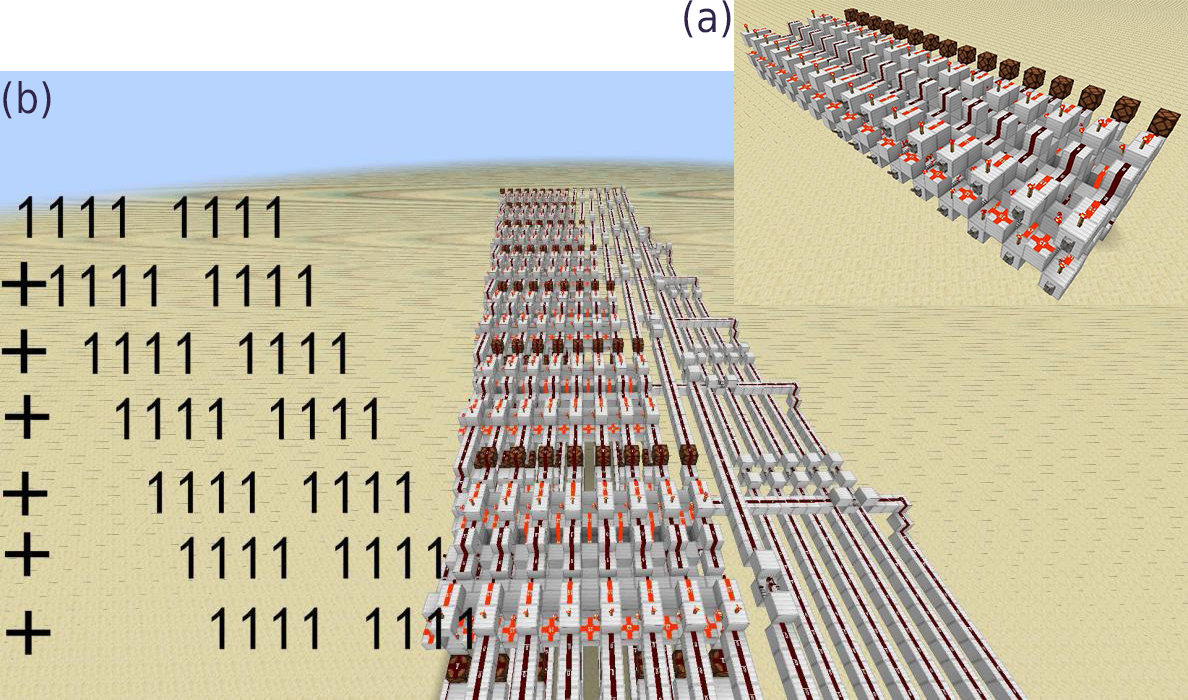
\includegraphics[width=0.85\linewidth]{common_multiplier_example.png}
        \caption{\small (a)单个16位全加器。(b)一般乘法器的结构。}
        \label{fig:ordinary-multiplier}
    \end{figure}

    第一步:将$a_1$与$a_2$,$a_3$与$a_4$,$a_5$与$a_6$,$a_7$与$a_8$分别使用全加器相加,得到结果分别记为$b_1,b_2,b_3,b_4$,这一步计算复杂度为$O(1)$.

    第二步:将$b_1$与$b_2$,$b_3$与$b_4$分别使用全加器相加,得到的结果记为$c_1$和$c_2$,这一步计算复杂度同样为$O(1)$。

    第三步:将$c_1$与$c_2$使用全加器相加得到结果$r$,这一步计算复杂度为$O(1)$。$r$是最终的乘法结果。总计算复杂度为$O(\log n)$。因为是8位乘法,故$n=8$。以2为底时,$\log_2n=3$,对应我们所需的三个步骤。

    \begin{figure}[h]
        \centering
        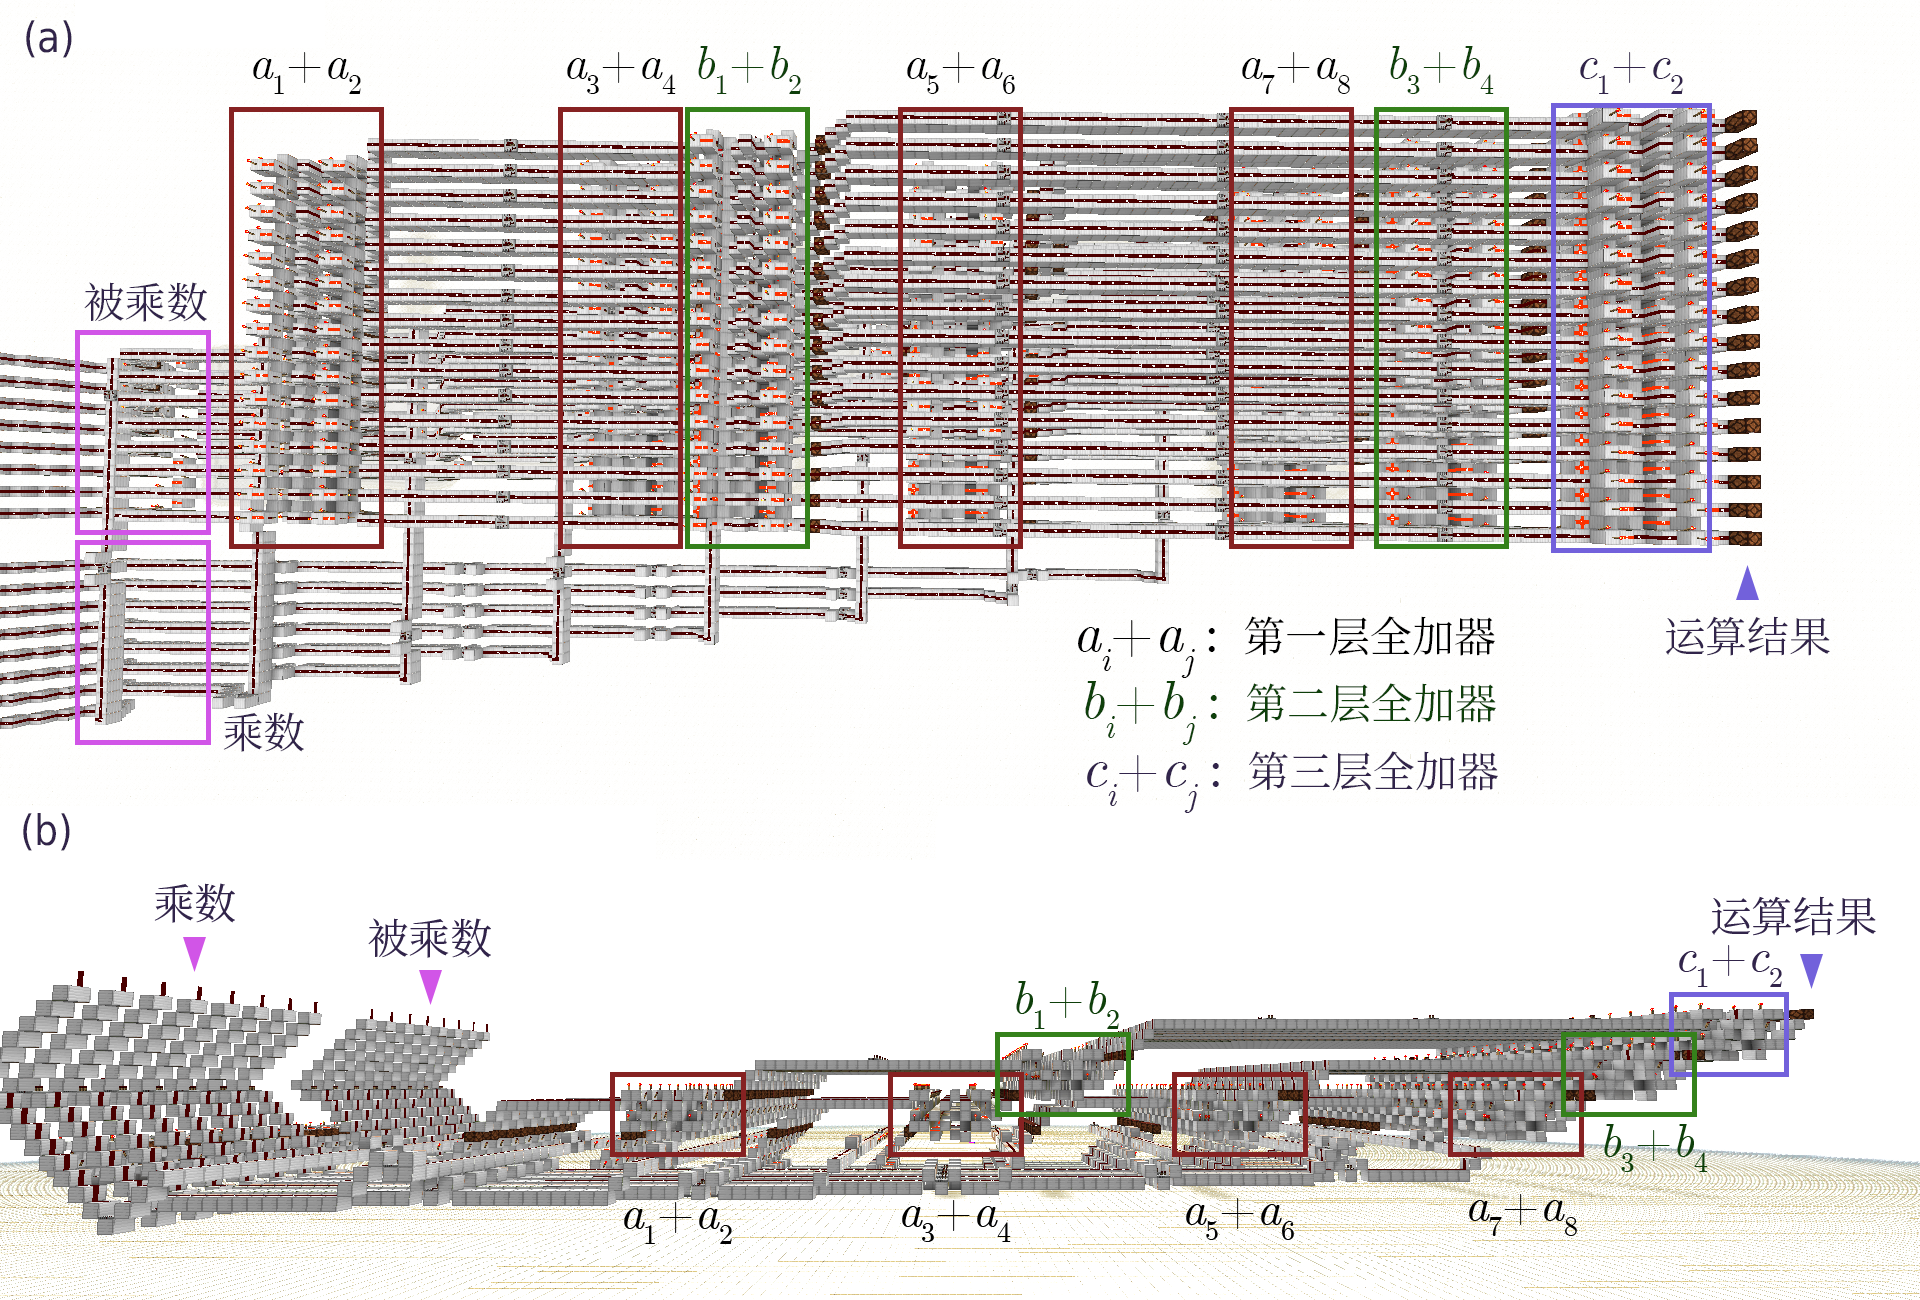
\includegraphics[width=0.97\linewidth]{overview.png}
        \caption{\small 树状乘法器的整体概览,(a)俯视图,(b)侧视图。}
        \label{fig:tree-multiplier-overview}
    \end{figure}

    树状乘法器有着更低的计算复杂度,并且建造难度较低,此外配合封闭进位加法器(CCA)可以获得更好的效果,这是红石计算器建造中可供选择的方案之一。

    最后感谢@辰占鳌头与@mail\_set的提醒与指导。

    \bibliographystyle{unsrt}
    \bibliography{reference}
    
\end{document}
